\documentclass{beamer}

%\includeonlyframes{current}

\usepackage[T1]{fontenc}
\usepackage[utf8]{inputenc}
\usepackage{unicode}
\usepackage[american]{babel}
\usepackage{amsmath,amssymb,amsthm}
\usepackage{tikz}
\usepackage[backend=biber,citestyle=authoryear-comp,bibstyle=beamer,doi=false,isbn=false,url=false,maxnames=10]{biblatex}
\bibliography{defeo}

\mode<presentation>{%
  \usetheme{Boadilla}
}
\beamertemplatenavigationsymbolsempty

\usepackage{sourcesanspro}
\usepackage[amssymb,amsfonts]{concmath}
\usefonttheme[onlymath]{serif}

\renewcommand{\emph}[1]{{\usebeamercolor[fg]{structure}#1}}

%\let\footcite\footnote

\newcommand{\C}{ℂ}
\newcommand{\R}{ℝ}
\newcommand{\Z}{ℤ}
\newcommand{\N}{ℕ}
\newcommand{\Q}{ℚ}
\newcommand{\F}{\mathbb{F}}
\renewcommand{\P}{\mathbb{P}}
\renewcommand{\O}{\mathcal{O}}
\newcommand{\tildO}{\mathcal{\tilde{O}}}
\newcommand{\End}{\operatorname{End}}
\newcommand{\chr}{\operatorname{char}}
\newcommand{\Cl}{\operatorname{Cl}}
\renewcommand{\a}{{\mathfrak{a}}}
\renewcommand{\b}{{\mathfrak{b}}}
\newcommand{\cyc}[1]{{〈 #1 〉}}
\newcommand{\ord}{\operatorname{ord}}

\usetikzlibrary{arrows,matrix,decorations,decorations.text,decorations.pathmorphing,calc}

\pgfkeys{/triangle/.code=\tikzset{x={(-0.5cm,-0.866cm)},y={(1cm,0cm)}}}
\pgfkeys{/lattice/.code n args={4}{\tikzset{cm={#1,#2,#3,#4,(0,0)}}}}

\newcommand{\axes}[4]{
  \clip (#1,#3) rectangle (#2,#4);
  \draw [thin, gray, -latex] (#1,0) -- (#2,0);% Draw x axis
  \draw [thin, gray, -latex] (0,#3) -- (0,#4);% Draw y axis
}

\newcommand{\lattice}[2]{
  \draw[style=help lines,dashed] (#1-1,#1-1) grid[step=1] (#2+1,#2+1);
  \foreach \x in {#1,...,#2}{
    \foreach \y in {#1,...,#2}{
      \node[draw,circle,inner sep=2pt,fill] at (\x,\y) {};
      % Places a dot at those points
    }
  }
}

\newcommand{\bl}[1]{\textcolor{blue}{#1}}
\newcommand{\rd}[1]{\textcolor{red}{#1}}
\newcommand{\gr}[1]{\textcolor{green}{#1}}

% This command defines a triangle of dots of given height
\newcommand{\dottriangle}[2][\i-\j]{%
  \foreach \i in {0,...,#2} {%
    \foreach \j in {0,...,\i} {%
      \draw(\i,\j) node{#1};%
    }%
  }}


\title{Isogeny graphs in cryptography}
\author[Luca De Feo]{Luca De Feo}
\date[Mar 18, 2019 --- Maths of PKC]{March 18, 2019\\
  \href{https://mathsofpkc.sciencesconf.org/}{Mathematical foundations of asymmetric cryptography}\\
  Aussois, Savoie
}
\institute[U Paris Saclay]{Université Paris Saclay, UVSQ}

\begin{document}

\frame[plain]{
  \begin{tikzpicture}[remember picture,overlay]
    \node[at=(current page.center), opacity=0.7] {
      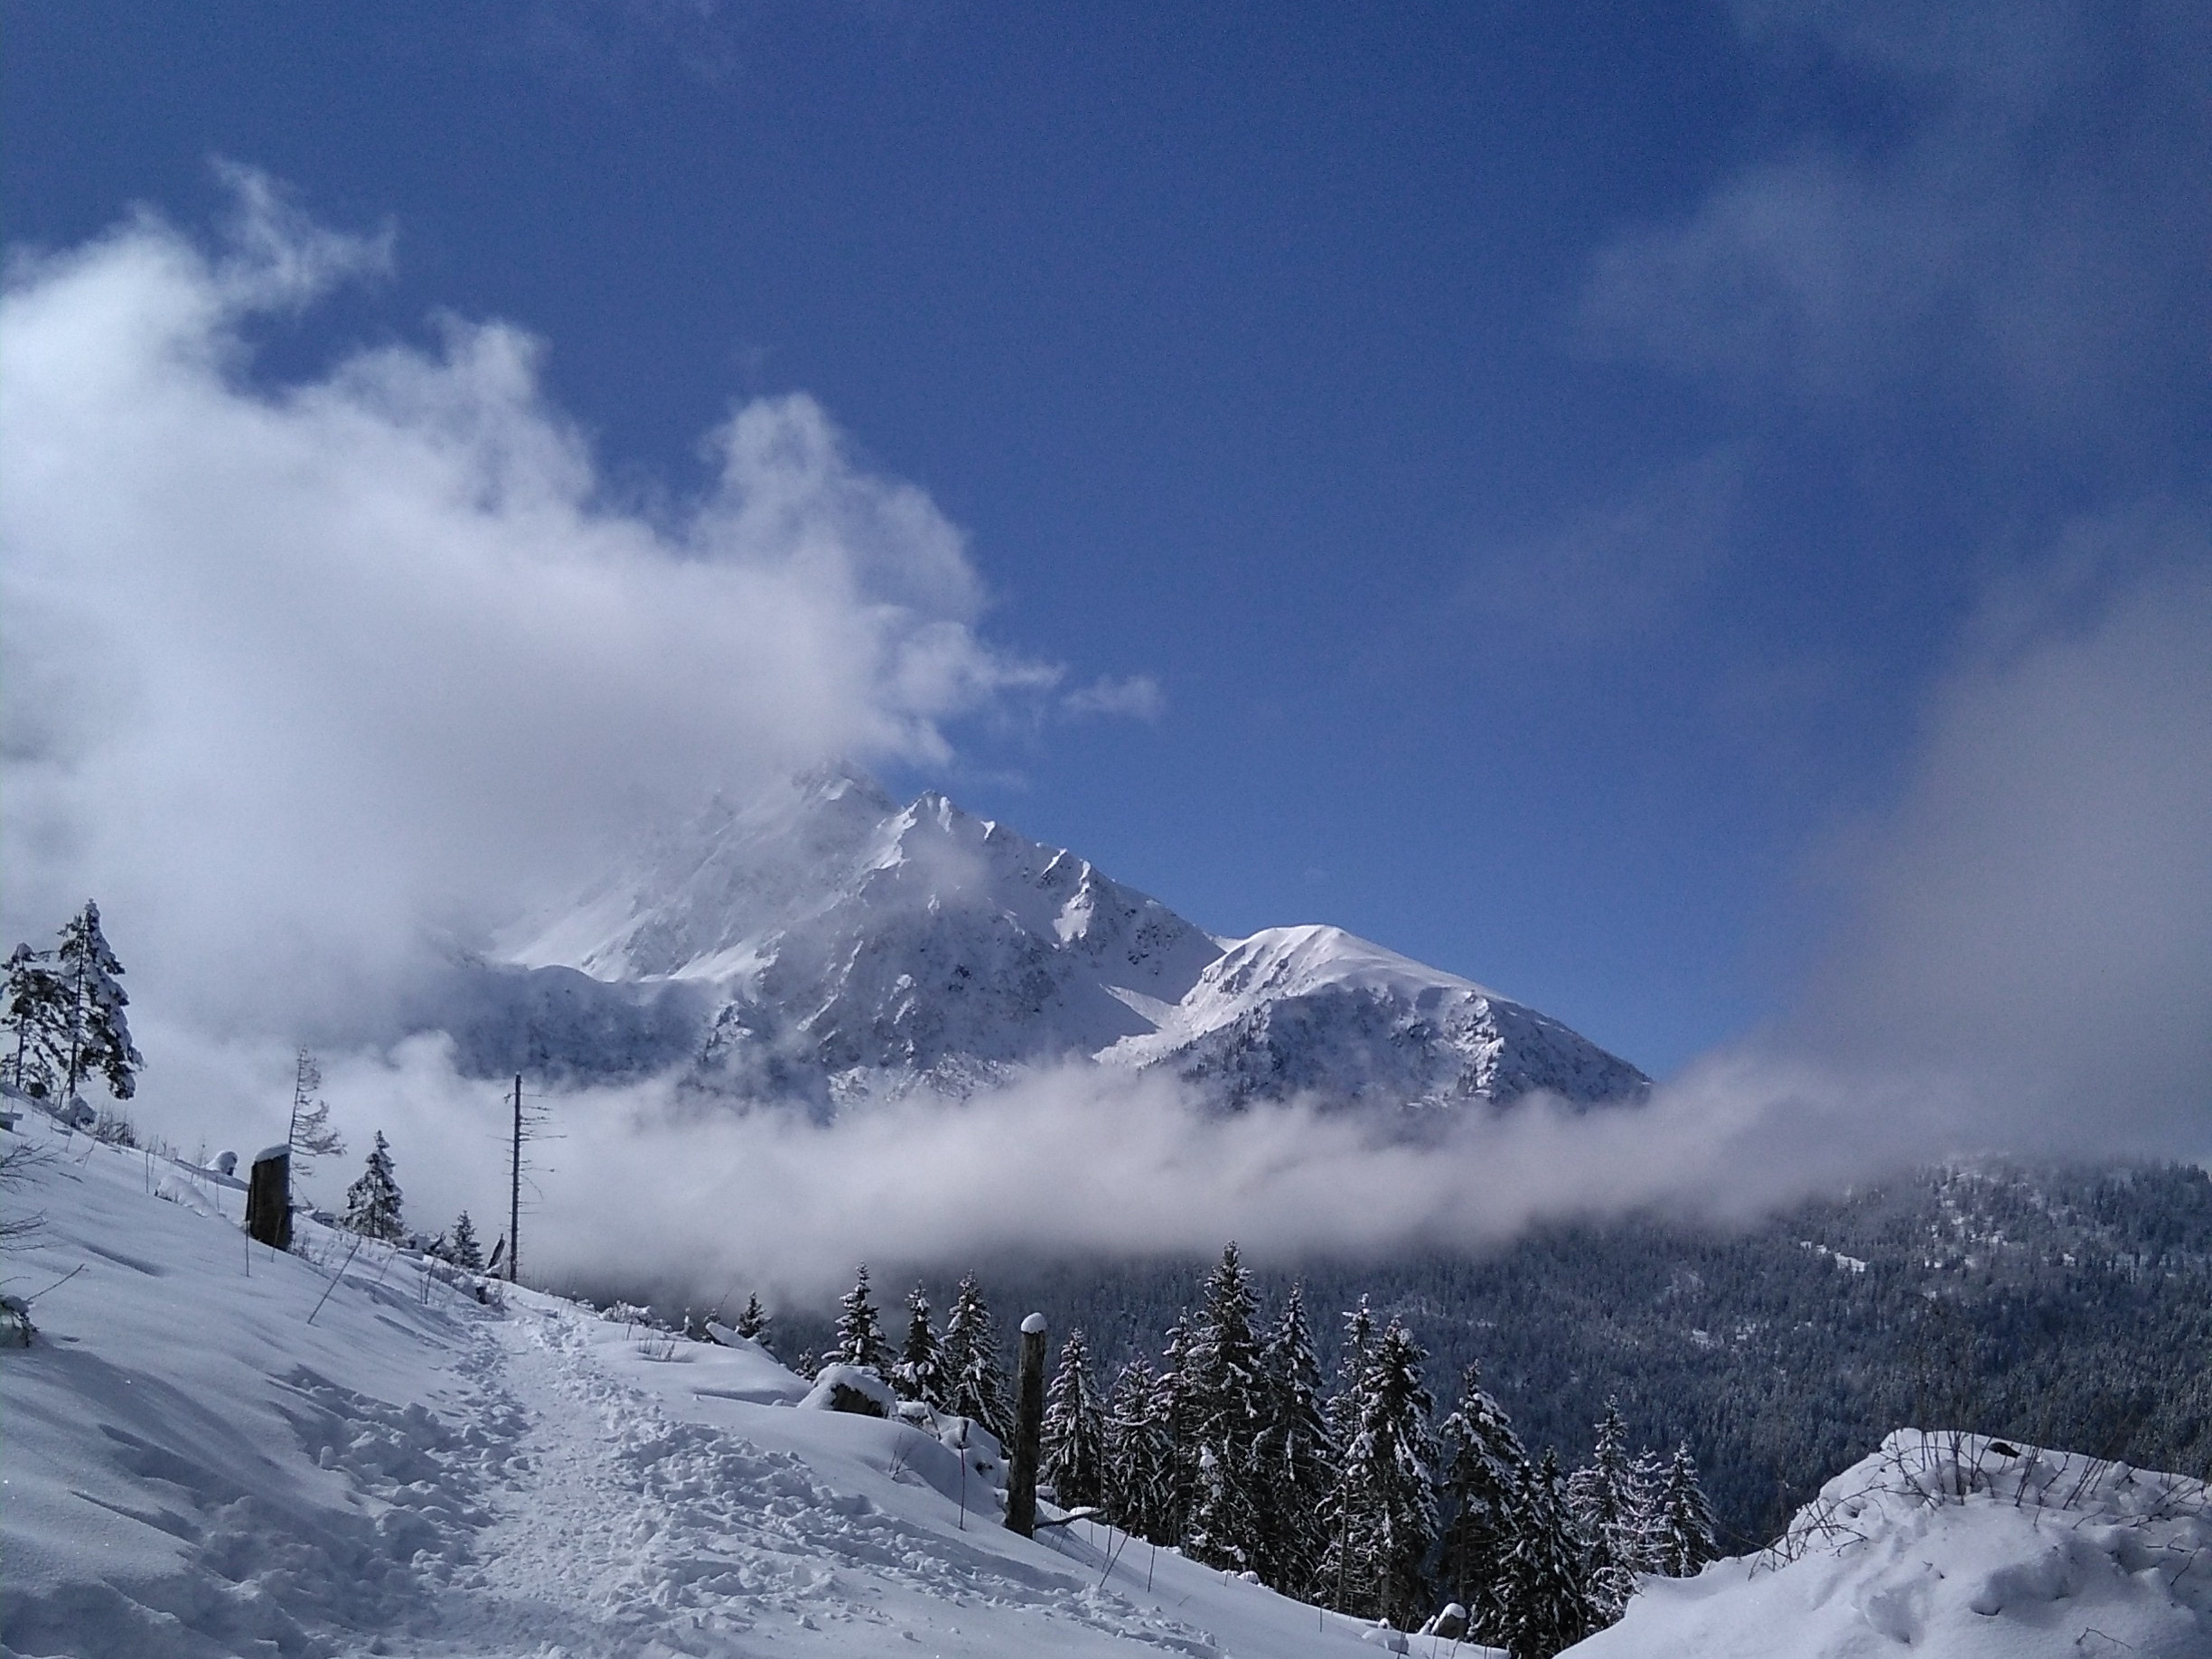
\includegraphics[width=1.2\paperwidth]{7laux.jpg}
    };
  \end{tikzpicture}
  \vspace{-1.1cm}
  {\bf \titlepage}
  \vspace{0.5cm}
  \begin{center}
    Slides online at~~~\emph{\url{http://defeo.lu/docet/}}
  \end{center}
}

%% 

\begin{frame}
  \frametitle{Overview}
  \tableofcontents  
\end{frame}

%%
%% 

\section{Isogeny graphs}

\subsection{Elliptic Curves}

\begin{frame}{Elliptic curves}
  \begin{columns}
    \begin{column}{0.4\textwidth}
      Let $k$ be a field of characteristic $\ne 2,3$.

      An \emph{elliptic curve \textit{defined over $k$}} is the locus
      in the \emph{projective space} $\P^2(\bar{k})$ of an equation
      \[\emph{Y^2Z = X^3 + aXZ^2 + bZ^3},\]
      where $a,b\in k$ and $4a^3+27b^2\ne 0$.

      \begin{itemize}
      \item<2-> $\O=(0:1:0)$ is the \emph{point at infinity};
      \item<3-> $y^2 = x^3 + ax + b$ is the \emph{affine Weierstrass equation}.
      \end{itemize}
    \end{column}
    \begin{column}{0.6\textwidth}
      \begin{center}
        \begin{tikzpicture}[domain=-2.4566:4,samples=100,yscale=1/2]
          \draw plot (\x,{sqrt(\x*\x*\x-4*\x+5)});
          \draw plot (\x,{-sqrt(\x*\x*\x-4*\x+5)});

          \draw[thin,gray,-latex] (0,-7) -- (0,7);
          \draw[thin,gray,-latex] (-3,0) -- (4,0);
        \end{tikzpicture}
      \end{center}
    \end{column}
  \end{columns}
\end{frame}

%%

\begin{frame}{The group law}
  \begin{columns}
    \begin{column}{0.4\textwidth}
      \begin{block}{Bezout's theorem}
        Every line cuts $E$ in exactly three points (counted with
        multiplicity).
      \end{block}

      Define a \emph{group law} such that any three colinear points
      add up to zero.

      \begin{itemize}
      \item<2-> The law is \emph{algebraic}\\ (it has \textit{formulas});
      \item<3-> The law is \emph{commutative};
      \item<3-> $\O$ is the \emph{group identity};
      \item<3-> \emph{Opposite points} have the same $x$-value.
      \end{itemize}
    \end{column}
    \begin{column}{0.6\textwidth}
      \begin{center}
        \begin{tikzpicture}[domain=-2.4566:4,samples=100,yscale=1/2]
          \draw plot (\x,{sqrt(\x*\x*\x-4*\x+5)});
          \draw plot (\x,{-sqrt(\x*\x*\x-4*\x+5)});

          \draw[thin,gray,-latex] (0,-7) -- (0,7);
          \draw[thin,gray,-latex] (-3,0) -- (4,0);
          \draw (-3,1) -- (4,8/3+3);
          \begin{scope}[every node/.style={draw,circle,inner sep=1pt,fill},cm={1,2/3,0,0,(0,3)}]
            \node at (-2.287980,0) {};
            \node at (-0.535051,0) {};
            \node at (3.267475,0) {};
          \end{scope}
          \begin{scope}[every node/.style={yshift=0.3cm},cm={1,2/3,0,0,(0,3)}]
            \node at (-2.287980,0) {$P$};
            \node at (-0.535051,0) {$Q$};
            \node at (3.267475,0) {$R$};
          \end{scope}

          \draw[dashed] (3.267475,3.267475*2/3+3) -- (3.267475,-3.267475*2/3-3) 
          node[draw,circle,inner sep=1pt,fill] {}
          node[xshift=-0.1cm,anchor=east] {$P+Q$};
        \end{tikzpicture}
      \end{center}
    \end{column}
  \end{columns}
\end{frame}

%%

\begin{frame}{Why should I care? (Diffie--Hellman key exchange)}
  \begin{description}
  \item[Goal:] Alice and Bob have never met before. They are chatting
    over a public channel, and want to agree on a \emph{shared secret}
    to start a private conversation.
  \item[Setup:] They agree on a (large) cyclic group $G=〈g〉$
    of (prime) order $q$.
  \end{description}

  \begin{center}
    \begin{tikzpicture}
      \node at (0,0) {\bf Alice};
      \node at (7,0) {\bf Bob};
      \node at (0,-1) {pick random \alert{$a∈ℤ/qℤ$}};
      \node at (0,-1.5) {compute $A=g^a$};
      \node at (7,-1) {pick random \alert{$b∈ℤ/qℤ$}};
      \node at (7,-1.5) {compute $B=g^b$};
      \draw[->]
      (1,-2) to node[auto] {$A$} (6,-2);
      \draw[->] (6,-2.5) to node[auto] {$B$} (1,-2.5);
      \node at (3.5,-3.5) {\emph{Shared secret} is \alert{$B^a=g^{ab}=A^b$}};
    \end{tikzpicture}
  \end{center}
\end{frame}

%%

\begin{frame}{Brief history of DH key exchange}
  \begin{description}
  \item[1976] Diffie \& Hellman publish \emph{New directions in
      cryptography}, suggest using $G=\F_p^\ast$.
  \item[1978] Pollard publishes his \emph{discrete logarithm}
    algorithm ($O(\sqrt{\# G})$ complexity).
  \item[1980] Miller and Koblitz independently suggest using
    \emph{elliptic curves} $G=E(\F_p)$.
  \item[1994] Shor publishes his quantum polynomial time
    \emph{discrete logarithm / factoring} algorithm.
  \item[2005] NSA standardizes elliptic curve key agreement (ECDH) and
    signatures ECDSA.
  \item[2017] $\sim 70\%$ of web traffic is secured by ECDH and/or
    ECDSA.
  \item[2017] NIST launches \emph{post-quantum competition}, says
    ``not to bother moving to elliptic curves, if you haven't yet''.
  \end{description}
\end{frame}

%% 

\begin{frame}{Why should I care? (cont'd)}

  {\large\emph{But, also:}}
  \begin{itemize}
  \item Elliptic Curve Factoring Method (Lenstra '85);
  \item Elliptic Curve Primality Proving (Atkin, Morain '86-'93);
  \item Efficient normal bases for finite fields (Couveignes, Lercier '10);
  \item \dots
  \end{itemize}
\end{frame}

%%

\begin{frame}{What are elliptic curves?}
  \begin{block}{For mathematicians}
    \begin{itemize}
    \item The \emph{smooth projective curves of genus 1};
    \item The simplest \emph{abelian varieties} (dimension 1);
    \item Finitely generated abelian groups of mysterious free rank
      (aka \emph{BSD conjecture});
    \item What you use to make examples.
    \end{itemize}
  \end{block}

  \pause
  
  \begin{block}{For cryptographers}
    \begin{itemize}
    \item \emph{Finite abelian} groups (often cyclic);
    \item ``2-dimensional'' generalizations of $μ_k$ (the \emph{roots
        of unity} of $k$);
    \item Boh
    \end{itemize}
  \end{block}
\end{frame}

%%

%%%%%%%%%%%%%%%%%%%%%%%%%%%%%%%%%%%%%%%
%%%%%%%%%%%%%%%%%%%%%%%%%%%%%%%%%%%%%%%

\subsection{Isogenies}

%%%%%%%%%%%%%%%%%%%%%%%%%%%%%%%%%%%%%%%
%%%%%%%%%%%%%%%%%%%%%%%%%%%%%%%%%%%%%%%

\subsection{Endomorphism rings}

%%%%%%%%%%%%%%%%%%%%%%%%%%%%%%%%%%%%%%%
%%%%%%%%%%%%%%%%%%%%%%%%%%%%%%%%%%%%%%%

\subsection{Isogeny graphs}


%%%%%%%%%%%%%%%%%%%%%%%%%%%%%%%%%%%%%%%%%%%%%%%%%%%%%%%%%%%%%%%%%%%%%%%%%%%%%
%%%%%%%%%%%%%%%%%%%%%%%%%%%%%%%%%%%%%%%%%%%%%%%%%%%%%%%%%%%%%%%%%%%%%%%%%%%%%

\section{Cryptography}

\subsection{Isogeny walks and Hash functions}

\begin{frame}{History of isogeny-based cryptography}
  \begin{description}
  \item[1996] Couveignes introduces the \emph{Hard Homogeneous
      Spaces (HHS)}. His work stays unpublished for 10 years.
  \item[2006] Rostovtsev \& Stolbunov independently rediscover
    Couveignes ideas, suggest isogeny-based Diffie--Hellman as a
    \emph{quantum-resistant} primitive.
  \item[2006-2010] Other isogeny-based protocols by Teske and Charles,
    Goren \& Lauter.
  \item[2011-2012] D., Jao \& Plût introduce \emph{SIDH}, an
    efficient post-quantum key exchange inspired by Couveignes,
    Rostovtsev, Stolbunov, Charles, Goren, Lauter.
  \item[2017] SIDH is submitted to the NIST competition (with the name
    \emph{SIKE}, only isogeny-based candidate).
  \item[2018] Castryck, Lange, Martindale, Panny \& Renes publish an
    efficient variant of HHS named \emph{CSIDH}.
  \item[2019] New isogeny protocols: Signatures, Verifiable Delay Functions, \dots
  \end{description}
\end{frame}


%%%%%%%%%%%%%%%%%%%%%%%%%%%%%%%%%%%%%%%
%%%%%%%%%%%%%%%%%%%%%%%%%%%%%%%%%%%%%%%

\subsection{Pairing verification and Verifiable Delay Functions}

%%%%%%%%%%%%%%%%%%%%%%%%%%%%%%%%%%%%%%%
%%%%%%%%%%%%%%%%%%%%%%%%%%%%%%%%%%%%%%%

\subsection{Key exchange}

%%%%%%%%%%%%%%%%%%%%%%%%%%%%%%%%%%%%%%%
%%%%%%%%%%%%%%%%%%%%%%%%%%%%%%%%%%%%%%%

\subsection{Proofs of knowledge and Signatures}

%%%%%%%%%%%%%%%%%%%%%%%%%%%%%%%%%%%%%%%
%%%%%%%%%%%%%%%%%%%%%%%%%%%%%%%%%%%%%%%

\subsection{Open Problems}


%%
%%

\begin{frame}[allowframebreaks]
  \frametitle{References}

  \defbibfilter{books}{\type{book} \or \type{booklet} \or \type{thesis}
    \or \type{report} \or \type{collection} \or \type{manual}
    \or \type{periodical} \or \type{proceedings}}
  \defbibfilter{articles}{\not \(\type{book} \or \type{booklet} \or \type{thesis}
    \or \type{report} \or \type{collection} \or \type{manual}
    \or \type{periodical} \or \type{proceedings}\)}

  \beamertemplatebookbibitems
  \printbibliography[filter=books]
  \beamertemplatearticlebibitems
  \printbibliography[filter=articles]
\end{frame}

\end{document}


% LocalWords:  Isogeny abelian isogenies hyperelliptic supersingular Frobenius
% LocalWords:  isogenous


